\section{AXI-Master interface}

The AXI-Master interface ({\tt AxiMst.vhd}) is the module in charge of writing to the AXI4-Stream bus. Since the MicroBlaze can read from the AXI4-Stream bus, the AXI-Master interface could be used to send data to the MicroBlaze from the IP-core of interest. The AXI-master block is shown in figure~\ref{f9}.

\begin{figure}[!h]
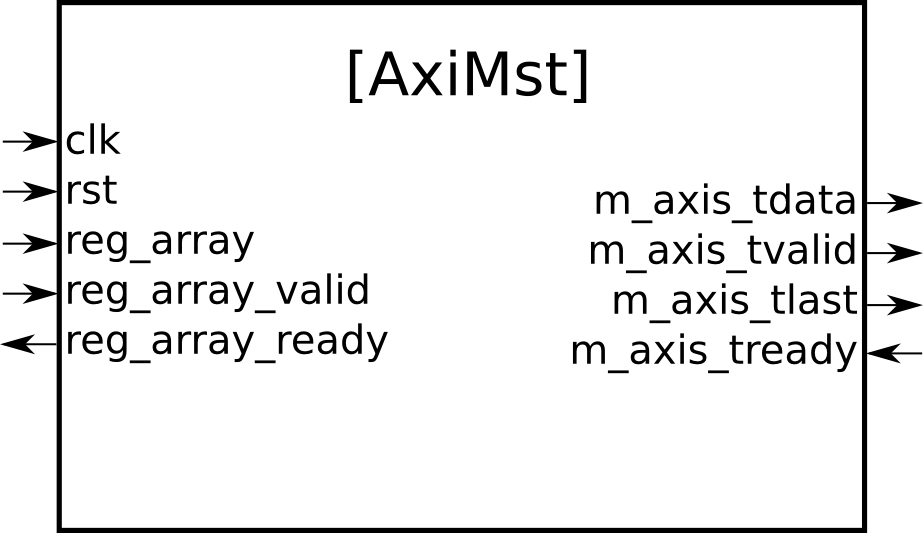
\includegraphics[scale=0.25]{images/axiMstBlock.png}
\caption{AXI-Master interface block}
\label{f9}
\end{figure}

Opposite to the AXI-Slave interface, the AXI-Master interface works as a Parallel-To-Serial interface. In other words, data will come in a parallel fashion through {\tt reg\_array} and place it serially over {\tt m\_axis\_tdata}. Loading the data in {\tt reg\_array} can be done by a valid signal called {\tt reg\_array\_valid}, and it must be set to '$1$' for data loading. In addition to a valid signal, a ready signal ({\tt reg\_array\_ready}) is used for stopping data loading when the interface is serializing and putting data on {\tt m\_axis\_tdata}. Furthermore, when ready signal is '$1$', the interface is ready for receiving data. Otherwise, the ready signal will be '$0$'.

How the data are arranged by the AXI-Master interface is shown in figure~\ref{f10}. Similar to the AXI-Slave interface, the WIDTH and NUM\_REG variables are generic and let users configure the interface as it is needed. Remember that AXI4-Stream work with $32$ bits, so WIDTH should be $32$. More details, will be covered by the application example in the next section.

\begin{figure}[!h]
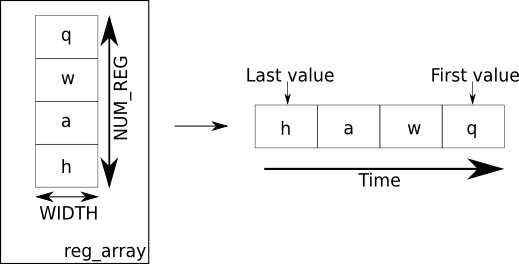
\includegraphics[scale=0.5]{images/axiMstReg.png}
\caption{AXI-Master register organization}
\label{f10}
\end{figure}

\subsection{Application example}

In the following application example, we will use AXI-Slave ({\tt AxiSlv.vhd}) and AXI-Master ({\tt AxiMst.vhd}) interfaces together with two RNG modules working in parallel. At the end of this application you should be able to adapt your own IP-core to work with the above mentioned interfaces.

First of all, a top module in VHDL is needed in order to connect all blocks. This top module should be as shown in the figure~\ref{f11}.  We are going to call this module as {\tt AxiTwoRng.vhd}. If you do not want to write the code, then look for the {\it AxiTwoRng} folder in the source repository.

\begin{figure}[!h]
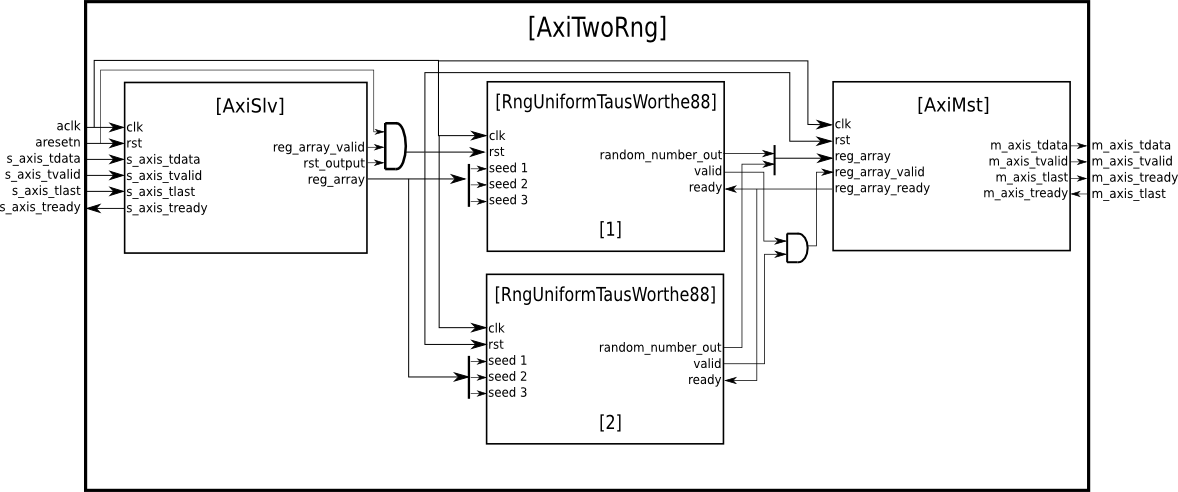
\includegraphics[scale=0.4]{images/axiTwoRngBlock.png}
\caption{AxiTwoRng.vhd}
\label{f11}
\end{figure}

Similarly to the application example of AXI-Slave, the RNG module is connected to the AXI-Slave. However, there are some additionally details. First, the {\tt reg\_array} signal will contain six seeds for the RNG modules, three seeds for each one. Secondly, the generic parameters for the {\tt AxiTwoRng.vhd} is used as follows:

\begin{itemize}
\item G\_RESET\_ACTIVE = 0
\item WIDTH = 32
\item NUM\_REG\_SLV = 6
\item NUM\_REG\_MST = 2
\item NUM\_RST\_CYCLE = 3
\end{itemize}

The number of registers (NUM\_REG\_SLV) is $6$, because as it is stated before we need six seeds. Here, it might be good to remember that the number of registers is named as NUM\_REG\_SLV and not as NUM\_REG. The main reason is that we need to make a difference between the number of registers for the Slave and Master interface. Therefore, the number of registers for the AXI-Master is given by NUM\_REG\_MST. Furthermore, since we are instantiating two RNG modules, the application will produce $64$ bits. Thus, the parameter NUM\_REG\_MST should be $2$. Finally, the number of clock cycles for the reset (NUM\_RST\_CYCLE) is $3$.

On the other hand, the AXI-Master can control the generation of random numbers by the {\tt reg\_array\_ready} signal. Meanwhile, each valid signal {\tt valid} of the RNG modules is connected through an AND gate to the {\tt reg\_array\_valid} port.

At this point, we should have the following source files:

\begin{itemize}
\item {\tt AxiTwoRng.vhd}
\item {\tt AxiSlv.vhd}
\item {\tt AxiMst.vhd} 
\item {\tt RngUniformTausworthe88.vhd}
\end{itemize}

From now on, it is advisable follow the same directions given by the application example for the AXI-Slave interface. However, here are some additional hints:

\begin{itemize}
\item The MPD file is the same used in the AxiRng application example, since the interface is the same.
\item The software program (.c) for the AxiTwoRng application example is shown in figure~\ref{f12}.
\item The output for this application example is shown in figure~\ref{f13}.
\end{itemize}

\begin{figure}[!h]
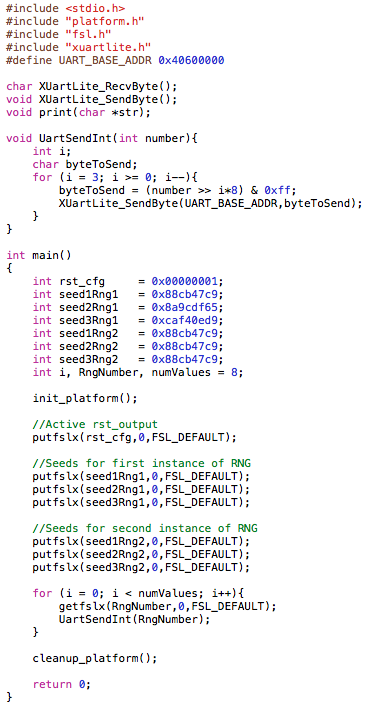
\includegraphics[scale=0.75]{images/axiTwoRngSwCode.png}
\caption{Source code for testing AxiTwoRng}
\label{f12}
\end{figure}

\begin{figure}[!h]
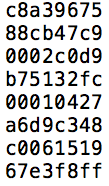
\includegraphics[scale=0.5]{images/twoRngVal.png}
\caption{First eight random values - AxiTwoRng}
\label{f13}
\end{figure}
